%MAKE ABSOLUTELY CERTAIN YOU ANONYMIZE DUMMY DESK REJECTIONS ARE FAIL

\documentclass[runningheads]{llncs}
%
\usepackage{amsmath}
\usepackage[T1]{fontenc}
% T1 fonts will be used to generate the final print and online PDFs,
% so please use T1 fonts in your manuscript whenever possible.
% Other font encodings may result in incorrect characters.
%
\usepackage{graphicx,verbatim}
% Used for displaying a sample figure. If possible, figure files should
% be included in EPS format.
%
% If you use the hyperref package, please uncomment the following two lines
% to display URLs in blue roman font according to Springer's eBook style:
%\usepackage{color}
%\renewcommand\UrlFont{\color{blue}\rmfamily}
%\urlstyle{rm}
%
\begin{document}
%
\title{Contributing Title}
%
\begin{comment}  %% Removed for anonymized MICCAI 2025 submission
\author{First Author\inst{1}\orcidID{0000-1111-2222-3333} \and
Second Author\inst{2,3}\orcidID{1111-2222-3333-4444} \and
Third Author\inst{3}\orcidID{2222--3333-4444-5555}}
%
\end{comment}

\author{Anon Authors}  %% Added for anonymized MICCAI 2025 submission
\authorrunning{Anonymized Author et al.}
\institute{Anonymized Affiliations \\
    \email{email@anonymized.com}}

    
\maketitle              % typeset the header of the contribution
%
\begin{abstract}
Accurately judging the depth of cerebral vessels is central to neurosurgical planning and image-guided navigation. One promising technology to assist in depth and placement determination is video-passthrough augmented reality headsets. This study seeks to determine whether depth-enhancement shaders improve depth perception when virtual anatomy is viewed against a real background. We present a 12 participant pilot study featuring a standalone MR application that anchors the virtual mesh to the real world coordinate and evaluates how participants' depth perception is influenced by three shaders that have been previously shown to contribute highly to depth perception: Phong (reference), aerial-perspective fog, and chromadepth. Participants were asked to correctly identify the middle depth point and then place a fiducial marker on the surface and then report their preferred shadings. Our finds show that while chromadepth is generally preferred by users and percieved as helpful, the measured effect of shaders in passthrough environments is negligible compared to parallax and occlusion.

\keywords{First keyword  \and Second keyword \and Another keyword.}


\end{abstract}
%
%
%
\section{Introduction}\label{sec:intro}
Neurovascular interventions, including the planning and clipping of aneurysms, the resection of arteriovenous malformations (AVMs), and the management of arteriovenous fistulae (AVFs), depend on a precise, three-dimensional understanding of how target vessels are situated within the surrounding brain~\cite{kersten-oertel_augmented_2015-1}. A central difficulty is judging the depth of a vessel of interest: it is typically embedded within, and partially occluded by, other anatomy, so its position relative to neighbouring vessels is hard to recover from the two-dimensional slices or flat desktop renderings used in conventional review, which provide weak and often ambiguous depth information~\cite{kersten-oertel_augmented_2015-1}. Video passthrough mixed reality (VPMR) is an appealing medium for this task: a head-mounted stereoscopic display supplies binocular disparity and head-coupled motion parallax, two strong depth cues, while registering the vasculature to the clinician's real workspace keeps the physical environment as context. 

 Given the wealth of research done on VR and AR depth perception cues and coloring, there is a gap in knowledge of if depth-enhancement shaders actually improve vessel depth judgement in a VPMR. On 2D displays and fixed overlays, cues such as aerial perspective (fog) and chromadepth substantially improve depth judgements of vascular data~\cite{kersten-oertel_evaluation_2014,ropinski_visually_2006}. In immersive VR, by contrast, binocular stereo and motion parallax are so strong that shader differences largely wash out~\cite{heinrich_estimating_2021,titov_effect_2021}. Passthrough MR sits between these regimes and adds its own difficulties: the virtual mesh competes with a real, textured background, and the passthrough imagery is geometrically distorted, reduced in resolution, and often suffers from the depth and occlusion problems long recognised in medical AR~\cite{macedo_occlusion_2023,adams_depth_2022}. Whether depth-enhancement shaders help depth judgement here or are largely washed out by stronger cues is therefore an open question we seek to help answer.

\noindent This study makes three contributions:
\begin{itemize}
  \item A standalone passthrough-MR system that registers a cerebral-vasculature mesh on the Meta Quest~3 and shades it appropriately while anchoring it to a known physical point in the room.
  \item A depth-placement task comparison of three depth-enhancement shaders: Phong, fog, and pseudo-chromadepth. Objective measurements collected from the placement task include accuracy, time to place, and the amount of user hand and head movements made while determining the depth.
  \item A study participant post-task survey to evaluate subjective measures including mental, physical, and temporal stress experiences as well as perceived effectiveness with each shader. \end{itemize}

\section{Related Work}\label{sec:related}

\subsubsection{Depth cues for vascular visualisation.}
For rendered vasculature, local (Phong) surface shading is the conventional illumination baseline. Added depth cues improve on it. Aerial perspective (fog) encodes distance as desaturation/attenuation of opacity over distance, and pseudo-chromadepth is a depth-to-colour ($\text{red}\rightarrow\text{blue}$) mapping introduced for angiography~\cite{ropinski_visually_2006}. These methods consistently rated among the strongest static cues for vascular data~\cite{kersten-oertel_evaluation_2014} and it has been adapted specifically to vascular \emph{surface} models~\cite{behrendt_combining_2017}. Depth-cue comparisons are well developed for surface renderings on conventional and VR displays~\cite{hombeck_evaluating_2022}, but have not been transferred to VPMR viewing of cerebral vasculature.

\subsubsection{Depth perception in immersive VR and the ceiling effect.}
Much of that evidence comes from 2D displays. In stereoscopic VR with free head movement, disparity and motion parallax are themselves powerful cues, and several studies report that shader choice then matters little: depth judgments of vascular models were more precise in VR than on desktop yet barely distinguished shading methods~\cite{heinrich_estimating_2021}, interactive cues had little impact on relative-depth perception for angiography volumes in VR~\cite{titov_effect_2021}, and, once camera motion is permitted, depth perception depends more on scene content than on the chosen technique~\cite{lesar_evaluation_2024}. This ceiling effect motivates our move to passthrough MR and requires that difficulty be raised deliberately. Methodologically, 3D-pointing studies show that error along the view/depth axis behaves differently from lateral error and is the axis on which depth cues act~\cite{teather_pointing_2011,batmaz_effect_2022}, motivating an error decomposition rather than a single 3D distance.

\subsubsection{Depth perception in passthrough augmented and mixed reality.}
Passthrough viewing changes the depth problem rather than easing it. The depth of virtual content overlaid on a real scene is systematically misperceived, modulated by display type, shadows, and relative position~\cite{adams_depth_2022} and by object shape, colour, and luminance~\cite{do_effects_2020}. These effects are acute for medical overlays, and depth-enhancing vascular visualisation has been pursued specifically for neurovascular AR~\cite{kersten-oertel_volume_2013,kersten-oertel_augmented_2015}. The closest prior work compares depth cues for vasculature but on desktop or tethered VR and with relative-depth or detection tasks~\cite{kersten-oertel_evaluation_2014,titov_effect_2021}, and we extend that comparison to standalone passthrough MR and to an in-scene target-placement task whose error is decomposed into depth and lateral components. 

\section{Methodology}\label{sec:related}
This study focuses on participant depth perception in a VPMR environment. In order to measure this, we present the user with a textured model of a brain based on the ICBM-152 composite. Nested inside of this model is nested a model of vasculature taken from anonymized TOF-MRA patient data(TODO: I need more info here - the scan I have just says Mumu's Data) registered to the ICBM-152 scan. The vasculature is shaded according to one of three conditions: 

\noindent This study makes three contributions:
\begin{itemize}
  \item Phong Shading: A reference baseline shading that does not change with proximity. In this study we used a red shading with a mild specular reflectivity.
  \item Fog Shading: A distance-based opacity shader that makes the structures closest to the center point more opaque and colored, while the color washes to a semi-transparent grey at a distance.
  \item Chromadepth: A distance based color gradient shader that colors the surfaces nearest to the reference point as red, and then steps through a color curve as the distance from the reference point increases.
  \end{itemize}

The shader's reference point was the tip of the virtual probe that extended from the motion controller. Upon bringing the probe to the brain model, a small hole opened in the brain model allowing them to see the inner vasculature model. Participants were asked to perform a sequence of six selection and six marking tasks in each shader. In the selection tasks, three points are placed in the vasculature. The participant was then required to select the point at the middle depth with the probe. Once the point was selected, the participant was asked to place a fiducial marker as close to the surface as they could without going too far into the surface by bringing the tip of the probe to the surface and pulling the trigger button. Participants were allowed to stand or sit, as well as move their head as much or as little as desired. 

During the selection and marking tasks, participant's selection correctness, movement range and viewing angle of the headset, marking accuracy and location are recorded. Upon finishing the selection and marking tasks, the participant is asked to complete a NASA TLX\cite{hart_development_1988} to review the shading conditions they encountered and give their preferences and subjective experiences with each shader. From these collected metrics and experiences, we can form a better picture of if the shading assisted in depth perception and what the magnitude of their impact was.

\section{User Study}
\subsection{Participant Demographics}
Participants were drawn from a non-clinical population on the rationale that the core depth judgement is a basic visual-system function and that prior work found similar novice/expert cue rankings for it~\cite{kersten-oertel_evaluation_2014}. The study was fully completed by 12 participants, 9 female and 3 male, while two participants stopped early due to motion sickness. Of the twelve, five were graduate students, one was a medical professional, while the other participants came from a wide array of professions. The majority of the participants(7) use VR headsets less than once a year, and the usages were primarily either video games or research. Most participants reported no familiarity with the brain anatomy(8), while three were somewhat familiar with brain anatomy and was professionally familiar.

\subsection{Data Preparation}
Each of the 12 participants completed 18 trials, giving 216 trials in total. Two trials recorded a
second placement seconds after the first, indicating a re-placement; for these we keep the first
placement only.

One block of three trials (one target, presented once under each shader) is excluded from all analyses,
leaving $12 \times 15 = 180$ trials in a balanced design of five targets per shader. The ground-truth
point for that block is not a plausible target: it lies 8.14\,cm from the nearest other point in the
stimulus, against a median nearest-neighbour spacing of 2.68\,cm among the remaining points. Because the
model is rigidly re-anchored in each session and distances are invariant under rigid transformation,
these two figures are identical to two decimal places for all twelve participants, which identifies the
cause as a single authoring fault in the stimulus rather than a per-session error. Consistent with this,
the block records 0/36 selection accuracy across every participant, which is a deterministic outcome
rather than a behavioural one. The exclusion is made on apparatus grounds and is independent of the
shader comparison, as the block was uniformly faulty in all three conditions.

Because $n=12$ and we do not assume the per-participant distributions are normal, we use Friedman
omnibus tests with Wilcoxon signed-rank post-hoc comparisons under Holm correction. We note that at
$n=12$ the smallest two-sided $p$ attainable by any distribution-free test is $2/2^{12}=0.00049$; we do
not report values below this floor, as they would reflect a parametric assumption rather than the data.

\subsection{Results}

\subsubsection{The task is depth-limited.}
A null result is only meaningful if the task was capable of showing an effect. We therefore first ask
whether placement error is dominated by depth at all, or is merely isotropic hand noise, which has no
preferred axis and so could not be reduced by any distance cue.

We decomposed each error vector in a view-aligned orthonormal frame, one axis along the view direction
and two perpendicular to it, and compared RMS error along each. This requires no distributional
assumption. Error along the view axis was 0.429\,cm against a per-axis lateral RMS of 0.193\,cm, a ratio
of 2.37 (median 2.41). The effect is unanimous: all twelve participants show depth error exceeding
lateral error (Wilcoxon signed-rank $W=0$, $p=0.00049$). The evidence here is the unanimity and the
magnitude of the ratio; the $p$-value only confirms that twelve out of twelve is not a coin flip. Depth
is thus roughly $2.4\times$ harder than the lateral axes in this task, as the 3D-pointing literature
predicts~\cite{teather_pointing_2011,batmaz_effect_2022}, and the task carries a large depth-specific
error component available for a shader to reduce.

\subsubsection{No shader affected performance.}
No shader reduced it. Table~\ref{tab:perf} reports every objective outcome recorded. None approaches
significance, and no pairwise contrast survives Holm correction.

\begin{table}[t]
\caption{Objective outcomes (per-participant means, $n=12$, 180 trials). Errors in cm, times in
seconds. Depth and lateral errors are computed on trials where the participant selected the designated
point. No outcome is significant.}\label{tab:perf}
\centering
\begin{tabular}{lcccc}
\hline\noalign{\smallskip}
Outcome & Phong & Fog & Chromadepth & Friedman \\
\noalign{\smallskip}\hline\noalign{\smallskip}
Selection accuracy      & 0.867 & 0.850 & 0.900 & $\chi^2=1.53$, $p=0.466$ \\
Depth error, unsigned   & 0.315 & 0.368 & 0.322 & $\chi^2=0.50$, $p=0.779$ \\
Lateral error           & 0.204 & 0.228 & 0.261 & $\chi^2=2.00$, $p=0.368$ \\
Depth error, signed     & $-0.069$ & $-0.167$ & $-0.036$ & $\chi^2=1.17$, $p=0.558$ \\
Time to place (s)       & 6.85  & 8.98  & 7.71  & $\chi^2=1.17$, $p=0.558$ \\
Time to select (s)      & 21.57 & 20.13 & 26.57 & $\chi^2=2.67$, $p=0.264$ \\
\noalign{\smallskip}\hline
\end{tabular}
\end{table}

Signed depth error was slightly negative in every condition (grand mean $-0.088$\,cm), the direction
expected for the depth compression characteristic of head-mounted displays, but did not differ
reliably from zero ($t=-1.45$, $p=0.174$).

Participants viewed the model freely, and did so extensively: head-position range over a session was a
median $2.08\times$ the full extent of the point cloud, and selection times reached 235\,s on individual
trials. The depth separation of the three candidate points, being a function of the vantage each
participant adopted rather than of the design, varied from 0.2 to 18.9\,cm across trials (median
4.0\,cm).

\subsubsection{But participants preferred chromadepth.}
Subjective responses diverge from performance. Asked which shader they found most helpful, 7 of the 10
participants who named a single condition chose chromadepth and 3 chose Phong; none chose fog (binomial
against $1/3$ chance, $p=0.020$). Counting the two further participants who named several conditions,
chromadepth was named by 9 of 12.

This item carries two caveats. The response options were edited partway through data collection, so one
condition appears under two labels, which we merged before tallying; and the item permitted multiple
selections rather than forcing a single choice. It is also one significant result among approximately
thirteen tests reported here, and would not survive Bonferroni correction across that set
($0.05/13 = 0.0038$). We therefore treat it as suggestive rather than confirmatory.

Workload responses corroborate the direction without reaching significance. On the NASA-TLX
subscales~\cite{hart_development_1988}, Phong was rated worst on all six (Table~\ref{tab:tlx}). Effort
is closest to significance ($p=0.063$). The subscales are mutually correlated, so their agreement is
corroborating rather than independent evidence; but the direction is unanimous across all six.

\begin{table}[t]
\caption{NASA-TLX subscales (per-participant means, $n=12$; higher is worse on every subscale). Phong is
rated worst on all six; none is significant.}\label{tab:tlx}
\centering
\begin{tabular}{lcccc}
\hline\noalign{\smallskip}
Subscale & Phong & Fog & Chromadepth & Friedman \\
\noalign{\smallskip}\hline\noalign{\smallskip}
Mental Demand   & 4.33 & 3.50 & 3.42 & $\chi^2=1.37$, $p=0.505$ \\
Physical Demand & 3.75 & 3.33 & 3.58 & $\chi^2=2.70$, $p=0.260$ \\
Temporal Demand & 2.25 & 1.92 & 1.50 & $\chi^2=3.56$, $p=0.168$ \\
Performance     & 3.83 & 3.42 & 3.50 & $\chi^2=1.15$, $p=0.562$ \\
Effort          & 4.17 & 3.50 & 3.42 & $\chi^2=5.52$, $p=0.063$ \\
Frustration     & 3.83 & 2.75 & 2.75 & $\chi^2=3.71$, $p=0.156$ \\
\noalign{\smallskip}\hline
\end{tabular}
\end{table}

\section{Discussion}

\subsubsection{Preference without benefit.}
Our participants preferred a shader that did not measurably help them. Chromadepth was named most
helpful by 9 of 12, and Phong was rated worst on all six NASA-TLX subscales, yet no shader moved any
objective outcome. This dissociation is the central result, and it is not an artefact of an insensitive
measure: the task carries a depth-specific error component roughly $2.4\times$ larger than its lateral
counterpart, in all twelve participants, so there was ample room for a distance cue to act.

\subsubsection{Why no effect?}
The most direct explanation lies in what our shaders encode. Both fog and chromadepth take the probe tip
as their reference point, so they encode \emph{distance from the instrument}, a quantity that is
radially symmetric about the tip. Our outcome, by contrast, is error along the \emph{view} axis. A
proximity encoding carries no information about which of two points lies further from the observer, and
so has no direct route to reducing view-axis error. This is a mismatch between manipulation and measure,
and it distinguishes our conditions from the view-dependent formulations of aerial perspective and
pseudo-chromadepth from which they take their colour mappings~\cite{ropinski_visually_2006}.

The null is nonetheless not vacuous, because a plausible indirect route existed and did not materialise.
During the marking task the candidate points are hidden but the vasculature remains shaded, so a
participant could advance the tip until the surface saturated toward the near end of the ramp and infer
contact from colour alone. Phong, which does not vary with proximity, offers no such signal. That
asymmetry could have produced a difference in placement accuracy. It did not.

A second account is that the task afforded strong native depth cues regardless. Viewing was
unconstrained: participants moved over a median head range of $2.08\times$ the extent of the point cloud
and took up to 235\,s per trial, and against world-locked anatomy such movement makes motion parallax
veridical and abundant. Prior work in immersive VR reports precisely this ceiling, with shader choice
mattering little once stereo and parallax are
available~\cite{heinrich_estimating_2021,titov_effect_2021,lesar_evaluation_2024}. Our data cannot
separate the two accounts, and they are not exclusive: a view-dependent shader might well have been
ceilinged by parallax even had we implemented one.

\subsubsection{Why, then, the preference?}
A cue can make a task feel easier without making it more accurate. That chromadepth was preferred while
Effort was the subscale nearest significance ($p=0.063$) suggests participants experienced a reduction in
the felt cost of a judgement they could make either way. For system design this is not nothing: a
visualisation that lowers perceived workload at no cost to accuracy may still merit adoption. But on
this evidence it should not be presented as an accuracy aid, and the gap between what users report and
what they achieve is itself a reason to measure both.

\subsection{Limitations}
Several limitations bound these conclusions.

\emph{Our shaders are not the view-dependent cues of the prior literature.} They adapt the colour
mappings of fog and pseudo-chromadepth to an instrument-proximity reference. Our results therefore speak
to proximity encodings and do not test whether view-dependent depth shaders help in passthrough MR,
which remains open.

\emph{Fog is confounded with occlusion.} It ramps opacity as well as colour, so the fog condition
renders vessels semi-transparent at distance and does not differ from Phong only in how distance is
encoded. Any fog effect, had we found one, could not have been attributed to the distance encoding
alone.

\emph{Viewing was unconstrained.} We neither restricted head movement nor imposed a response deadline,
so we cannot separate ``shaders do not help here'' from ``shaders do not help when parallax is freely
available''. The latter regime is arguably the clinically relevant one: a surgeon at a fixed vantage
over a craniotomy cannot orbit the anatomy.

\emph{The selection stage is not a depth measure.} The instruction to select the point ``in the middle''
does not specify middle \emph{in depth}, and because viewing was free, the depth separation of the three
candidates was set by each participant's vantage rather than by the design, ranging from 0.2 to
18.9\,cm. On some trials the candidates were effectively coplanar in depth. Selection accuracy is
reported descriptively only.

\emph{The sample is small and the study exploratory.} With $n=12$ and no pre-registration we can claim
only that we could not detect a difference, not that none exists. The preference result is one
significant test among many and requires independent confirmation.

\emph{The scene is fully virtual and the model a composite.} No physical object was present; the anchor
world-locks the model and supplies parallax, but not a real surface at a known distance. One patient's
vessels affinely registered to a template brain is adequate for perceptual work but is not
patient-specific anatomy.

\section{Conclusion}


\noindent Displayed equations are centered and set on a separate
line.
\begin{equation}
x + y = z
\end{equation}
Please try to avoid rasterized images for line-art diagrams and
schemas. Whenever possible, use vector graphics instead (see
Fig.~\ref{fig1}).

\begin{figure}
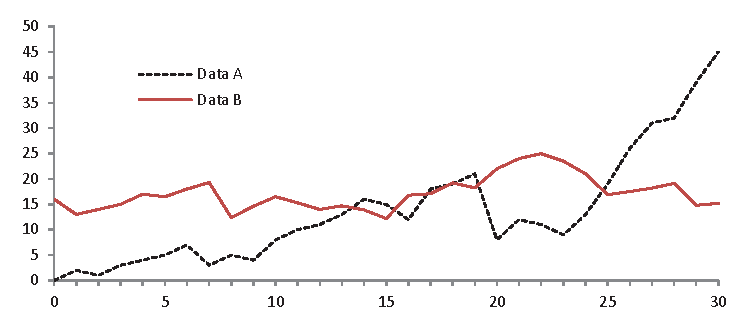
\includegraphics[width=\textwidth]{fig1.eps}
\caption{A figure caption is always placed below the illustration.
Please note that short captions are centered, while long ones are
justified by the macro package automatically.} \label{fig1}
\end{figure}

\begin{theorem}
This is a sample theorem. The run-in heading is set in bold, while
the following text appears in italics. Definitions, lemmas,
propositions, and corollaries are styled the same way.
\end{theorem}

\begin{proof}
Proofs, examples, and remarks have the initial word in italics,
while the following text appears in normal font.
\end{proof}
For citations of references, we prefer the use of square brackets
and consecutive numbers. Citations using labels or the author/year
convention are also acceptable. The following bibliography provides
a sample reference list with entries for journal
articles~\cite{ref_article1}, an LNCS chapter~\cite{ref_lncs1}, a
book~\cite{ref_book1}, proceedings without editors~\cite{ref_proc1},
and a homepage~\cite{ref_url1}. Multiple citations are grouped
\cite{ref_article1,ref_lncs1,ref_book1},
\cite{ref_article1,ref_book1,ref_proc1,ref_url1}.

\begin{comment}  

%% removed to make this anonymous :)
    
\begin{credits}
\subsubsection{\ackname} A bold run-in heading in small font size at the end of the paper is
used for general acknowledgments, for example: This study was funded
by X (grant number Y).

\subsubsection{\discintname}
It is now necessary to declare any competing interests or to specifically
state that the authors have no competing interests. Please place the
statement with a bold run-in heading in small font size beneath the
(optional) acknowledgments\footnote{If EquinOCS, our proceedings submission
system, is used, then the disclaimer can be provided directly in the system.},
for example: The authors have no competing interests to declare that are
relevant to the content of this article. Or: Author A has received research
grants from Company W. Author B has received a speaker honorarium from
Company X and owns stock in Company Y. Author C is a member of committee Z.
\end{credits}

\end{comment}
%
% ---- Bibliography ----
\bibliographystyle{splncs04}
\bibliography{zotero}

\end{document}
